\hypertarget{Predict_8c}{
\section{Predict.c File Reference}
\label{Predict_8c}\index{Predict.c@{Predict.c}}
}
{\tt \#include \char`\"{}party.h\char`\"{}}\par


Include dependency graph for Predict.c:\nopagebreak
\begin{figure}[H]
\begin{center}
\leavevmode
\includegraphics[width=420pt]{Predict_8c__incl}
\end{center}
\end{figure}
\subsection*{Functions}
\begin{CompactItemize}
\item 
void \hyperlink{Predict_8c_daf8a0eb8790ebf14f0e265de164d50e}{C\_\-splitnode} (SEXP node, SEXP learnsample, SEXP control)
\item 
SEXP \hyperlink{Predict_8c_dcd61d38c7c43d241d09a600b70fe3c5}{C\_\-get\_\-node} (SEXP subtree, SEXP newinputs, double mincriterion, int numobs)
\item 
SEXP \hyperlink{Predict_8c_dec31e3aa985e0af16ccaeac31237640}{R\_\-get\_\-node} (SEXP subtree, SEXP newinputs, SEXP mincriterion, SEXP numobs)
\item 
SEXP \hyperlink{Predict_8c_201fdee9dc7e3e71e90ea6609ed353cb}{C\_\-get\_\-nodebynum} (SEXP subtree, int nodenum)
\item 
SEXP \hyperlink{Predict_8c_4a30a8aa916f294059b6e2cbcb9e29d5}{R\_\-get\_\-nodebynum} (SEXP subtree, SEXP nodenum)
\item 
SEXP \hyperlink{Predict_8c_c4f4e806a78c376b13802ed2cf1e7b65}{C\_\-get\_\-prediction} (SEXP subtree, SEXP newinputs, double mincriterion, int numobs)
\item 
SEXP \hyperlink{Predict_8c_cbb3e45d03e1b544c94bf639b191a953}{C\_\-get\_\-nodeweights} (SEXP subtree, SEXP newinputs, double mincriterion, int numobs)
\item 
int \hyperlink{Predict_8c_d9d49b6a210f5c09a2a1d1aa496859ce}{C\_\-get\_\-nodeID} (SEXP subtree, SEXP newinputs, double mincriterion, int numobs)
\item 
SEXP \hyperlink{Predict_8c_c0668d268fe5a4bad29fbf4ead39c526}{R\_\-get\_\-nodeID} (SEXP tree, SEXP newinputs, SEXP mincriterion)
\item 
void \hyperlink{Predict_8c_ac36eff20575604b5d7558d512601d64}{C\_\-predict} (SEXP tree, SEXP newinputs, double mincriterion, SEXP ans)
\item 
SEXP \hyperlink{Predict_8c_9a5170a24bc00b727527b80cec5ca60a}{R\_\-predict} (SEXP tree, SEXP newinputs, SEXP mincriterion)
\item 
void \hyperlink{Predict_8c_8964e7493ed9cb96c271b168b721e329}{C\_\-getpredictions} (SEXP tree, SEXP where, SEXP ans)
\item 
SEXP \hyperlink{Predict_8c_a508a31f1fd7cd3668ad81eb0d00dd66}{R\_\-getpredictions} (SEXP tree, SEXP where)
\item 
SEXP \hyperlink{Predict_8c_4f6966402677cec07284a3e1bc25660f}{R\_\-predictRF\_\-weights} (SEXP forest, SEXP where, SEXP weights, SEXP newinputs, SEXP mincriterion, SEXP oobpred)
\item 
SEXP \hyperlink{Predict_8c_3be1a8f3155b0481350cecd4c094a416}{R\_\-proximity} (SEXP where)
\end{CompactItemize}


\subsection{Detailed Description}
Node splitting and prediction

\begin{Desc}
\item[Author:]\end{Desc}
\begin{Desc}
\item[Author]hothorn \end{Desc}
\begin{Desc}
\item[Date:]\end{Desc}
\begin{Desc}
\item[Date]2008-06-26 11:33:11 +0200 (Thu, 26 Jun 2008) \end{Desc}


Definition in file \hyperlink{Predict_8c-source}{Predict.c}.

\subsection{Function Documentation}
\hypertarget{Predict_8c_dcd61d38c7c43d241d09a600b70fe3c5}{
\index{Predict.c@{Predict.c}!C\_\-get\_\-node@{C\_\-get\_\-node}}
\index{C\_\-get\_\-node@{C\_\-get\_\-node}!Predict.c@{Predict.c}}
\subsubsection[C\_\-get\_\-node]{\setlength{\rightskip}{0pt plus 5cm}SEXP C\_\-get\_\-node (SEXP {\em subtree}, \/  SEXP {\em newinputs}, \/  double {\em mincriterion}, \/  int {\em numobs})}}
\label{Predict_8c_dcd61d38c7c43d241d09a600b70fe3c5}


Get the terminal node for obs. number `numobs' of `newinputs' \par
 \begin{Desc}
\item[Parameters:]
\begin{description}
\item[{\em subtree}]a tree \item[{\em newinputs}]an object of class `VariableFrame' \item[{\em mincriterion}]overwrites mincriterion used for tree growing \item[{\em numobs}]observation number \end{description}
\end{Desc}
\begin{Desc}
\item[\hyperlink{todo__todo000002}{Todo}]handle surrogate splits \end{Desc}


Definition at line 120 of file Predict.c.

References C\_\-i\_\-in\_\-set(), get\_\-missings(), get\_\-variable(), has\_\-missings(), S3get\_\-leftnode(), S3get\_\-maxcriterion(), S3get\_\-nodeterminal(), S3get\_\-primarysplit(), S3get\_\-rightnode(), S3get\_\-splitpoint(), S3get\_\-sumweights(), S3get\_\-surrogatesplits(), S3get\_\-toleft(), S3get\_\-variableID(), and S3is\_\-ordered().

Referenced by C\_\-get\_\-nodeID(), C\_\-get\_\-nodeweights(), C\_\-get\_\-prediction(), and R\_\-get\_\-node().

Here is the call graph for this function:\nopagebreak
\begin{figure}[H]
\begin{center}
\leavevmode
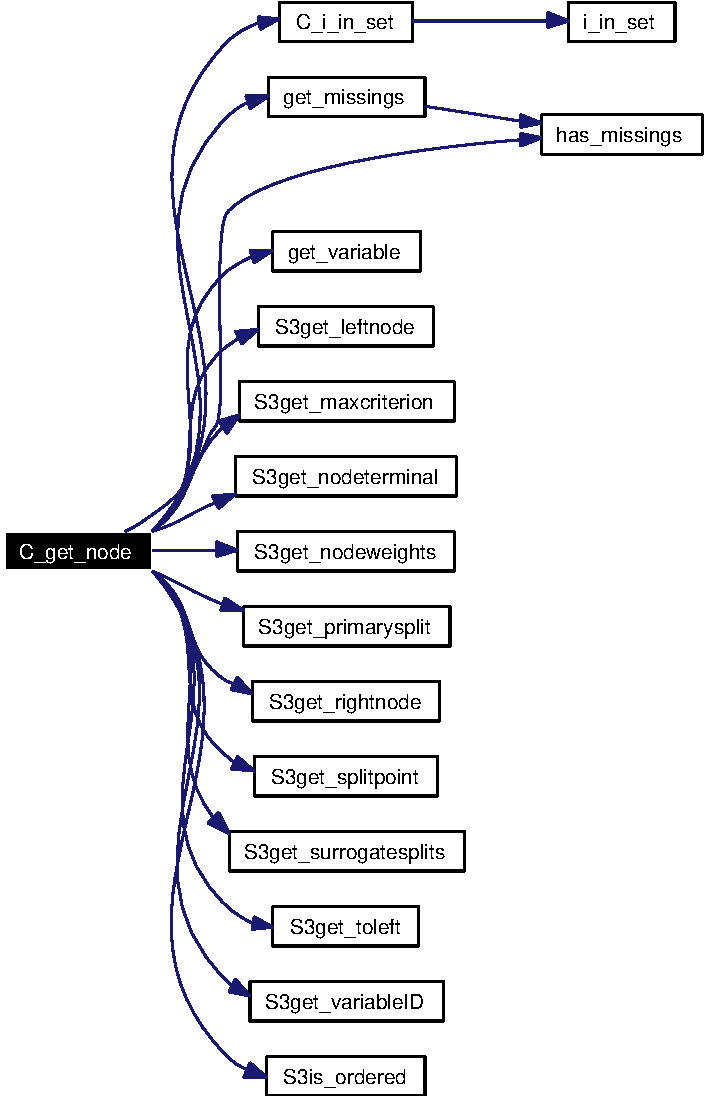
\includegraphics[width=186pt]{Predict_8c_dcd61d38c7c43d241d09a600b70fe3c5_cgraph}
\end{center}
\end{figure}
\hypertarget{Predict_8c_201fdee9dc7e3e71e90ea6609ed353cb}{
\index{Predict.c@{Predict.c}!C\_\-get\_\-nodebynum@{C\_\-get\_\-nodebynum}}
\index{C\_\-get\_\-nodebynum@{C\_\-get\_\-nodebynum}!Predict.c@{Predict.c}}
\subsubsection[C\_\-get\_\-nodebynum]{\setlength{\rightskip}{0pt plus 5cm}SEXP C\_\-get\_\-nodebynum (SEXP {\em subtree}, \/  int {\em nodenum})}}
\label{Predict_8c_201fdee9dc7e3e71e90ea6609ed353cb}


Get the node with nodeID `nodenum' \par
 \begin{Desc}
\item[Parameters:]
\begin{description}
\item[{\em subtree}]a tree \item[{\em nodenum}]a nodeID \end{description}
\end{Desc}


Definition at line 243 of file Predict.c.

References S3get\_\-leftnode(), S3get\_\-nodeID(), S3get\_\-nodeterminal(), and S3get\_\-rightnode().

Referenced by C\_\-getpredictions(), R\_\-get\_\-nodebynum(), and R\_\-predictRF\_\-weights().

Here is the call graph for this function:\nopagebreak
\begin{figure}[H]
\begin{center}
\leavevmode
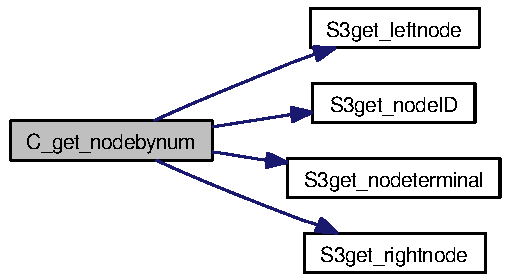
\includegraphics[width=140pt]{Predict_8c_201fdee9dc7e3e71e90ea6609ed353cb_cgraph}
\end{center}
\end{figure}
\hypertarget{Predict_8c_d9d49b6a210f5c09a2a1d1aa496859ce}{
\index{Predict.c@{Predict.c}!C\_\-get\_\-nodeID@{C\_\-get\_\-nodeID}}
\index{C\_\-get\_\-nodeID@{C\_\-get\_\-nodeID}!Predict.c@{Predict.c}}
\subsubsection[C\_\-get\_\-nodeID]{\setlength{\rightskip}{0pt plus 5cm}int C\_\-get\_\-nodeID (SEXP {\em subtree}, \/  SEXP {\em newinputs}, \/  double {\em mincriterion}, \/  int {\em numobs})}}
\label{Predict_8c_d9d49b6a210f5c09a2a1d1aa496859ce}


Get the nodeID for a new observation \par
 \begin{Desc}
\item[Parameters:]
\begin{description}
\item[{\em subtree}]a tree \item[{\em newinputs}]an object of class `VariableFrame' \item[{\em mincriterion}]overwrites mincriterion used for tree growing \item[{\em numobs}]observation number \end{description}
\end{Desc}


Definition at line 307 of file Predict.c.

References C\_\-get\_\-node(), and S3get\_\-nodeID().

Referenced by R\_\-get\_\-nodeID(), and R\_\-predictRF\_\-weights().

Here is the call graph for this function:\nopagebreak
\begin{figure}[H]
\begin{center}
\leavevmode
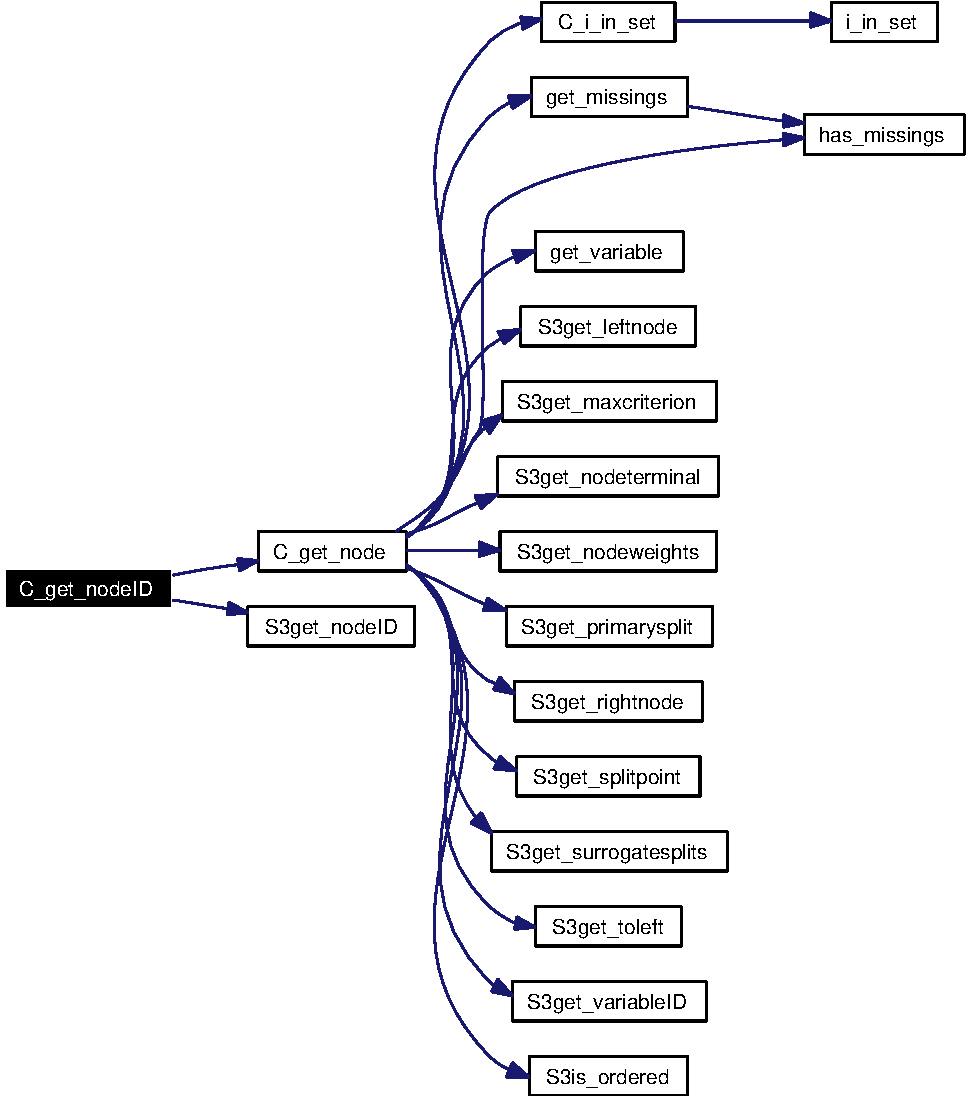
\includegraphics[width=248pt]{Predict_8c_d9d49b6a210f5c09a2a1d1aa496859ce_cgraph}
\end{center}
\end{figure}
\hypertarget{Predict_8c_cbb3e45d03e1b544c94bf639b191a953}{
\index{Predict.c@{Predict.c}!C\_\-get\_\-nodeweights@{C\_\-get\_\-nodeweights}}
\index{C\_\-get\_\-nodeweights@{C\_\-get\_\-nodeweights}!Predict.c@{Predict.c}}
\subsubsection[C\_\-get\_\-nodeweights]{\setlength{\rightskip}{0pt plus 5cm}SEXP C\_\-get\_\-nodeweights (SEXP {\em subtree}, \/  SEXP {\em newinputs}, \/  double {\em mincriterion}, \/  int {\em numobs})}}
\label{Predict_8c_cbb3e45d03e1b544c94bf639b191a953}


Get the weights for a new observation \par
 \begin{Desc}
\item[Parameters:]
\begin{description}
\item[{\em subtree}]a tree \item[{\em newinputs}]an object of class `VariableFrame' \item[{\em mincriterion}]overwrites mincriterion used for tree growing \item[{\em numobs}]observation number \end{description}
\end{Desc}


Definition at line 292 of file Predict.c.

References C\_\-get\_\-node(), and S3get\_\-nodeweights().

Here is the call graph for this function:\nopagebreak
\begin{figure}[H]
\begin{center}
\leavevmode
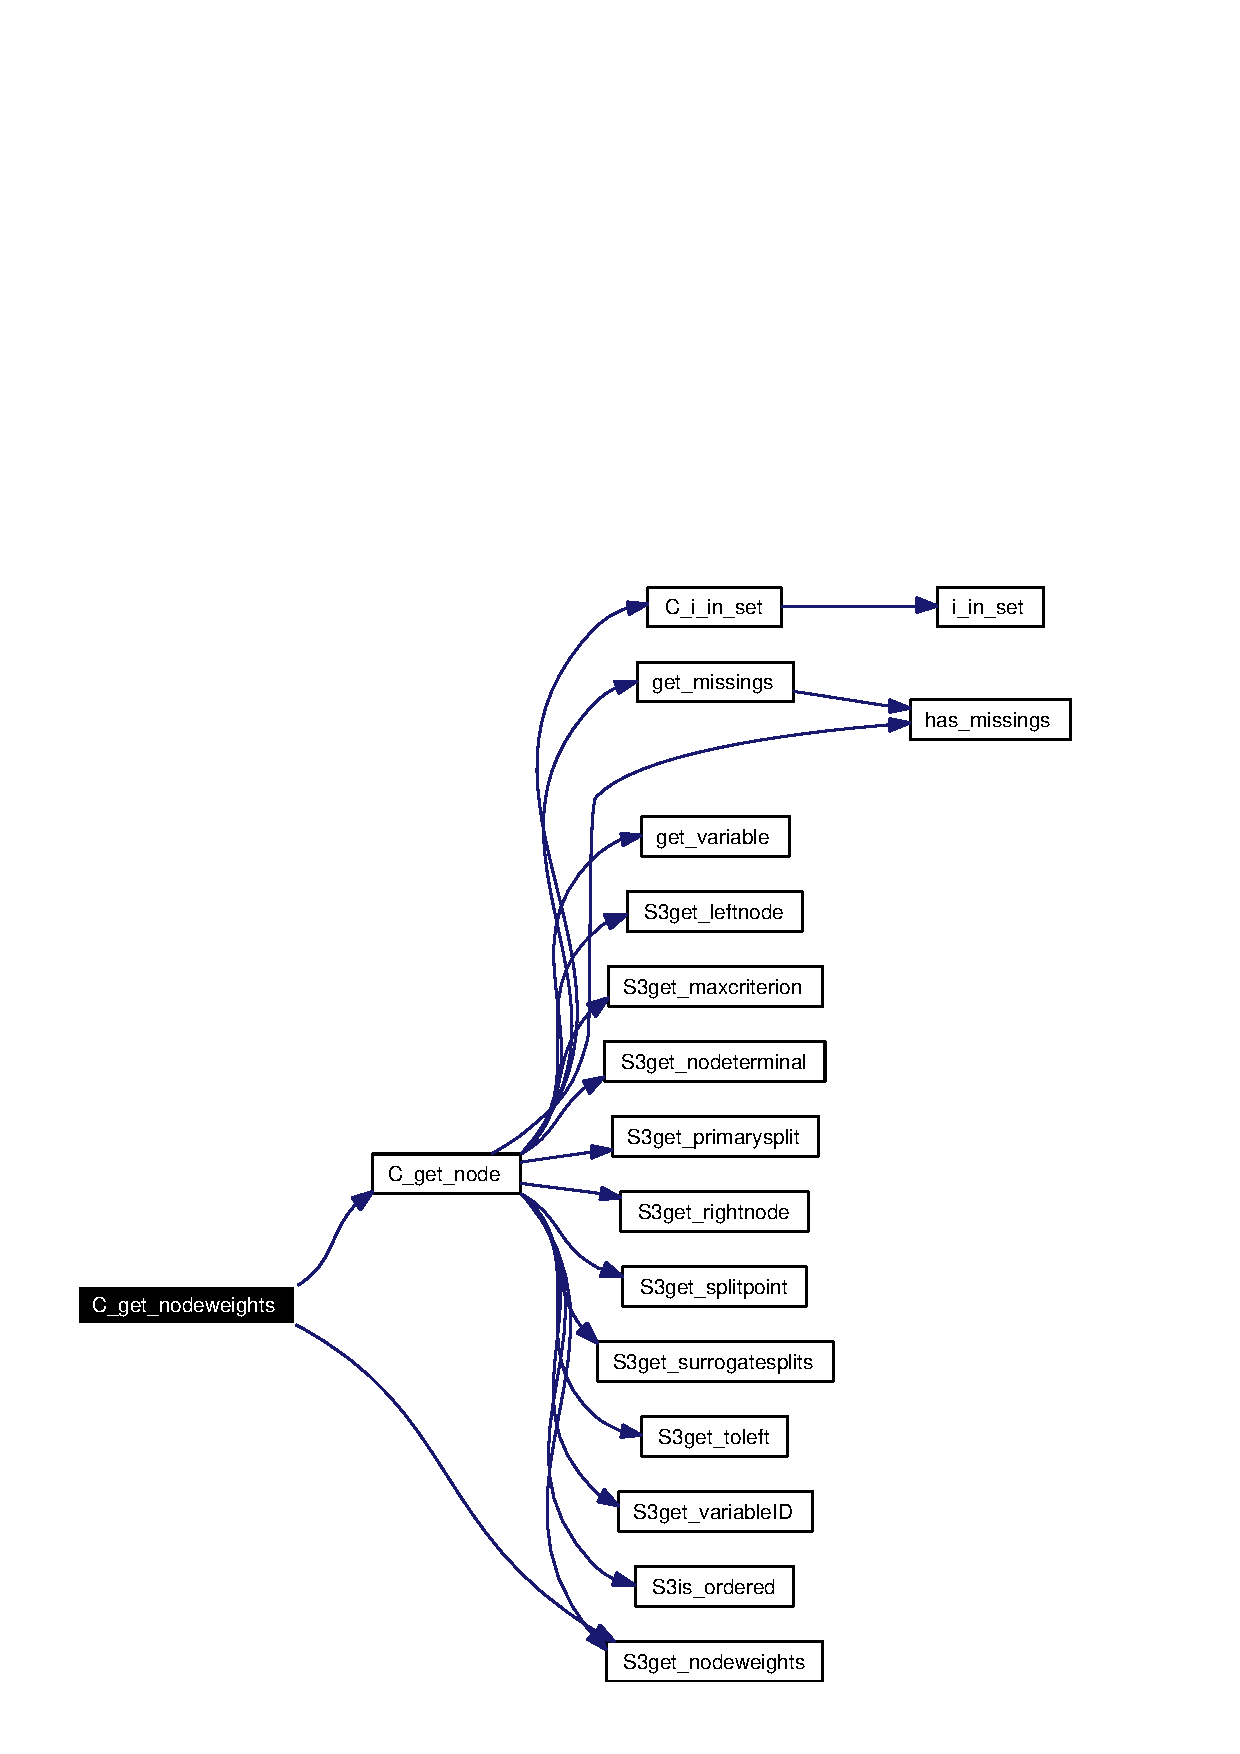
\includegraphics[width=272pt]{Predict_8c_cbb3e45d03e1b544c94bf639b191a953_cgraph}
\end{center}
\end{figure}
\hypertarget{Predict_8c_c4f4e806a78c376b13802ed2cf1e7b65}{
\index{Predict.c@{Predict.c}!C\_\-get\_\-prediction@{C\_\-get\_\-prediction}}
\index{C\_\-get\_\-prediction@{C\_\-get\_\-prediction}!Predict.c@{Predict.c}}
\subsubsection[C\_\-get\_\-prediction]{\setlength{\rightskip}{0pt plus 5cm}SEXP C\_\-get\_\-prediction (SEXP {\em subtree}, \/  SEXP {\em newinputs}, \/  double {\em mincriterion}, \/  int {\em numobs})}}
\label{Predict_8c_c4f4e806a78c376b13802ed2cf1e7b65}


Get the prediction of a new observation\par
 \begin{Desc}
\item[Parameters:]
\begin{description}
\item[{\em subtree}]a tree \item[{\em newinputs}]an object of class `VariableFrame' \item[{\em mincriterion}]overwrites mincriterion used for tree growing \item[{\em numobs}]observation number \end{description}
\end{Desc}


Definition at line 277 of file Predict.c.

References C\_\-get\_\-node(), and S3get\_\-prediction().

Referenced by C\_\-predict().

Here is the call graph for this function:\nopagebreak
\begin{figure}[H]
\begin{center}
\leavevmode
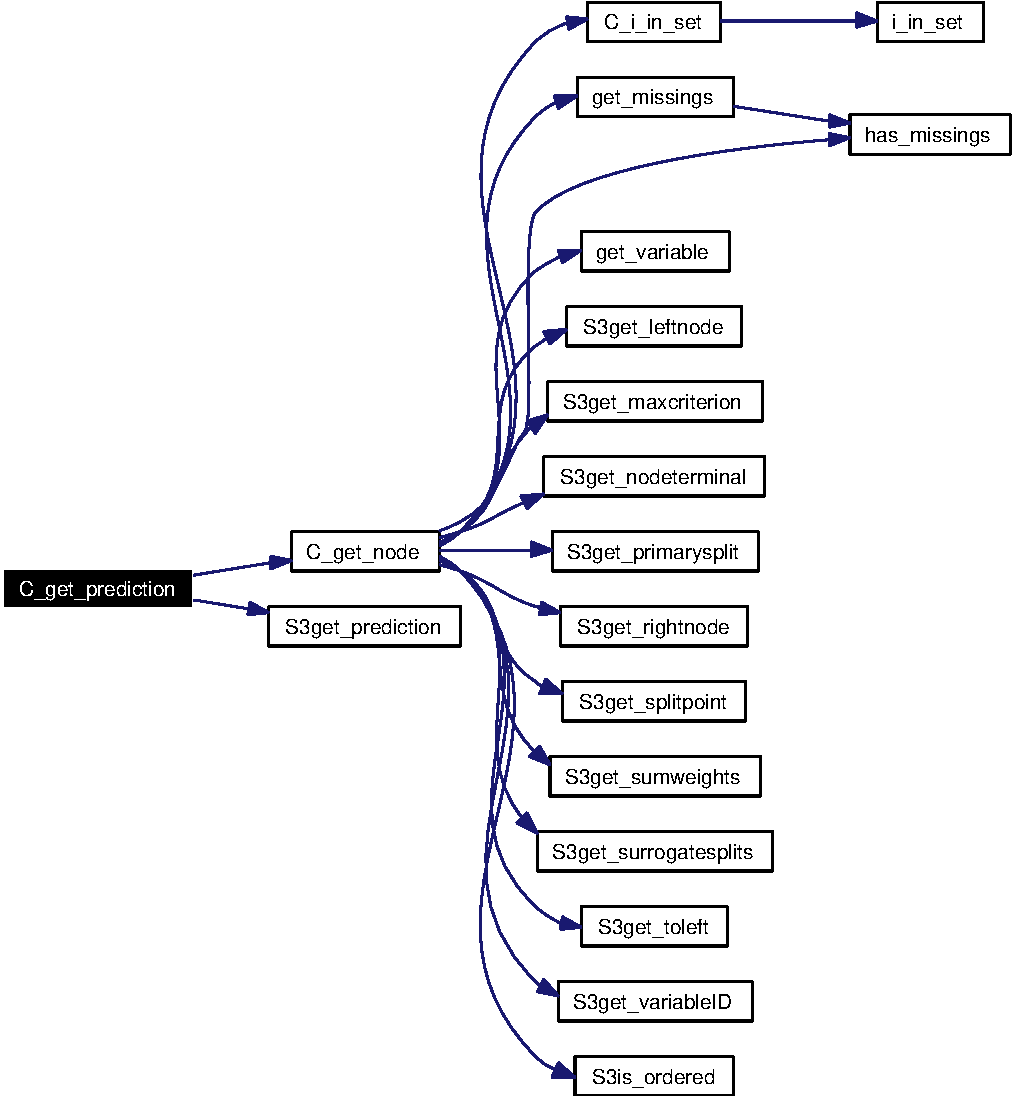
\includegraphics[width=260pt]{Predict_8c_c4f4e806a78c376b13802ed2cf1e7b65_cgraph}
\end{center}
\end{figure}
\hypertarget{Predict_8c_8964e7493ed9cb96c271b168b721e329}{
\index{Predict.c@{Predict.c}!C\_\-getpredictions@{C\_\-getpredictions}}
\index{C\_\-getpredictions@{C\_\-getpredictions}!Predict.c@{Predict.c}}
\subsubsection[C\_\-getpredictions]{\setlength{\rightskip}{0pt plus 5cm}void C\_\-getpredictions (SEXP {\em tree}, \/  SEXP {\em where}, \/  SEXP {\em ans})}}
\label{Predict_8c_8964e7493ed9cb96c271b168b721e329}


Get the predictions from `where' nodes\par
 \begin{Desc}
\item[Parameters:]
\begin{description}
\item[{\em tree}]a tree \item[{\em where}]vector of nodeID's \item[{\em ans}]return value \end{description}
\end{Desc}


Definition at line 385 of file Predict.c.

References C\_\-get\_\-nodebynum(), and S3get\_\-prediction().

Referenced by R\_\-getpredictions().

Here is the call graph for this function:\nopagebreak
\begin{figure}[H]
\begin{center}
\leavevmode
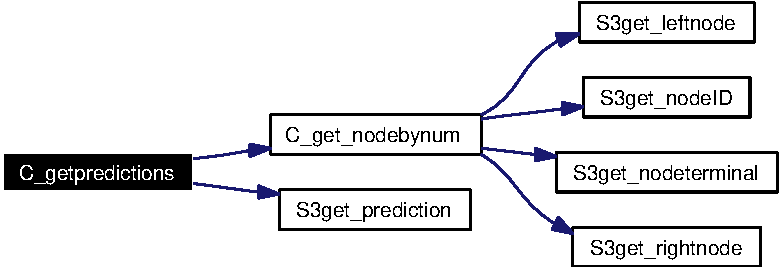
\includegraphics[width=203pt]{Predict_8c_8964e7493ed9cb96c271b168b721e329_cgraph}
\end{center}
\end{figure}
\hypertarget{Predict_8c_ac36eff20575604b5d7558d512601d64}{
\index{Predict.c@{Predict.c}!C\_\-predict@{C\_\-predict}}
\index{C\_\-predict@{C\_\-predict}!Predict.c@{Predict.c}}
\subsubsection[C\_\-predict]{\setlength{\rightskip}{0pt plus 5cm}void C\_\-predict (SEXP {\em tree}, \/  SEXP {\em newinputs}, \/  double {\em mincriterion}, \/  SEXP {\em ans})}}
\label{Predict_8c_ac36eff20575604b5d7558d512601d64}


Get all predictions for `newinputs' \par
 \begin{Desc}
\item[Parameters:]
\begin{description}
\item[{\em tree}]a tree \item[{\em newinputs}]an object of class `VariableFrame' \item[{\em mincriterion}]overwrites mincriterion used for tree growing \item[{\em ans}]return value \end{description}
\end{Desc}


Definition at line 344 of file Predict.c.

References C\_\-get\_\-prediction(), and get\_\-nobs().

Referenced by R\_\-predict().

Here is the call graph for this function:\nopagebreak
\begin{figure}[H]
\begin{center}
\leavevmode
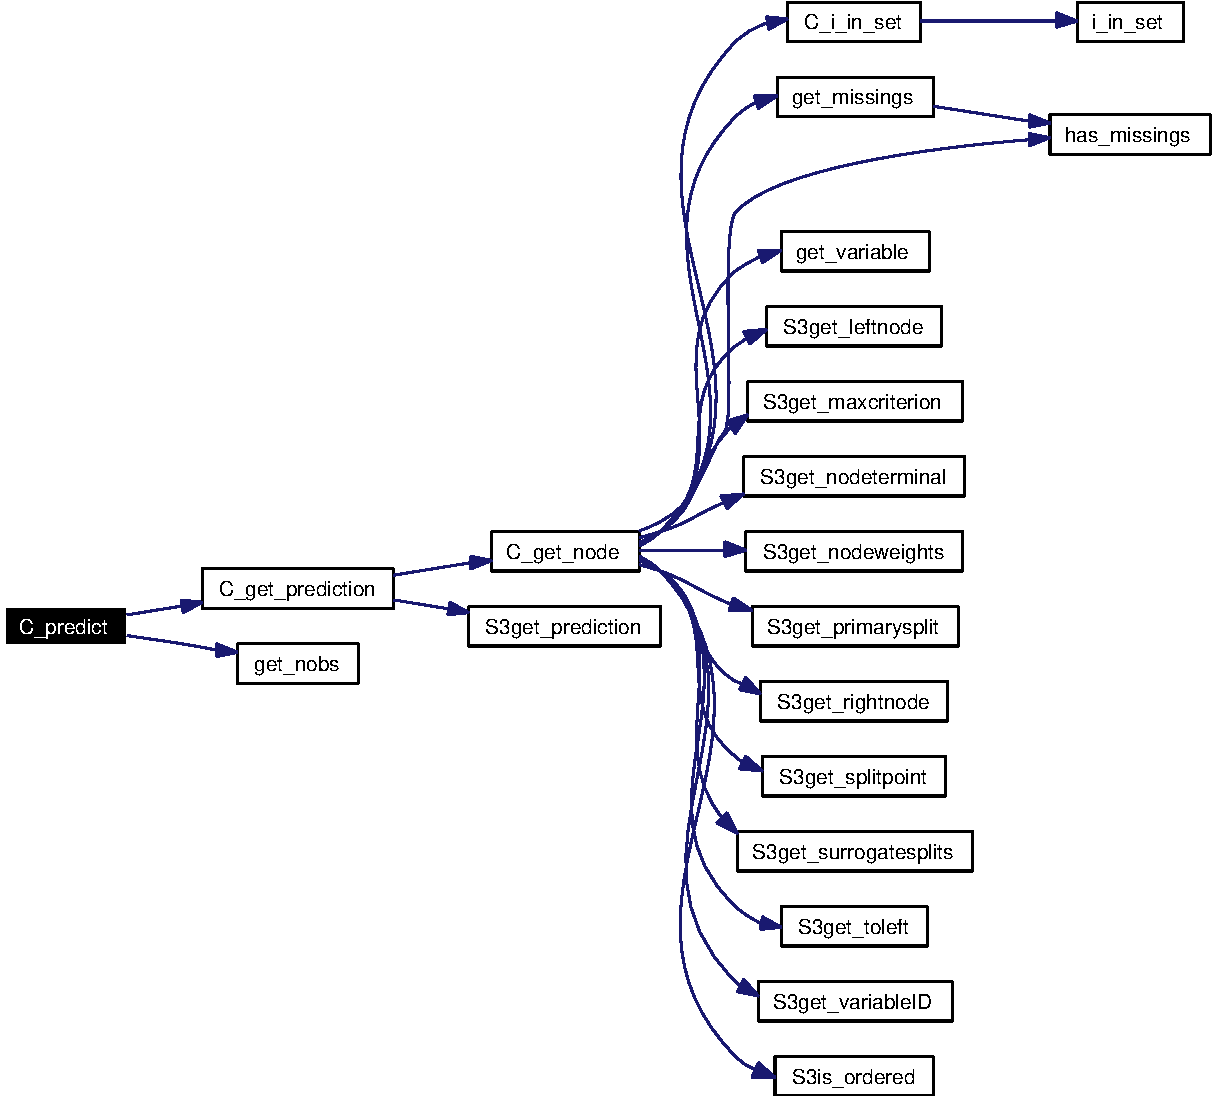
\includegraphics[width=307pt]{Predict_8c_ac36eff20575604b5d7558d512601d64_cgraph}
\end{center}
\end{figure}
\hypertarget{Predict_8c_daf8a0eb8790ebf14f0e265de164d50e}{
\index{Predict.c@{Predict.c}!C\_\-splitnode@{C\_\-splitnode}}
\index{C\_\-splitnode@{C\_\-splitnode}!Predict.c@{Predict.c}}
\subsubsection[C\_\-splitnode]{\setlength{\rightskip}{0pt plus 5cm}void C\_\-splitnode (SEXP {\em node}, \/  SEXP {\em learnsample}, \/  SEXP {\em control})}}
\label{Predict_8c_daf8a0eb8790ebf14f0e265de164d50e}


Split a node according to a splitting rule \par
 \begin{Desc}
\item[Parameters:]
\begin{description}
\item[{\em node}]the current node with primary split specified \item[{\em learnsample}]learning sample \item[{\em control}]an object of class `TreeControl' \end{description}
\end{Desc}
\begin{Desc}
\item[\hyperlink{todo__todo000001}{Todo}]outplace the splitting since there are at least 3 functions with nearly identical code \end{Desc}


Definition at line 21 of file Predict.c.

References C\_\-init\_\-node(), get\_\-maxsurrogate(), get\_\-missings(), get\_\-ninputs(), get\_\-nobs(), get\_\-predict\_\-trafo(), get\_\-splitctrl(), get\_\-variable(), has\_\-missings(), i\_\-in\_\-set(), ncol(), NODE\_\-LENGTH, PL2\_\-inputsSym, PL2\_\-responsesSym, S3\_\-LEFT, S3\_\-RIGHT, S3get\_\-nodeweights(), S3get\_\-primarysplit(), S3get\_\-splitpoint(), S3get\_\-variableID(), and S3is\_\-ordered().

Referenced by C\_\-TreeGrow().

Here is the call graph for this function:\nopagebreak
\begin{figure}[H]
\begin{center}
\leavevmode
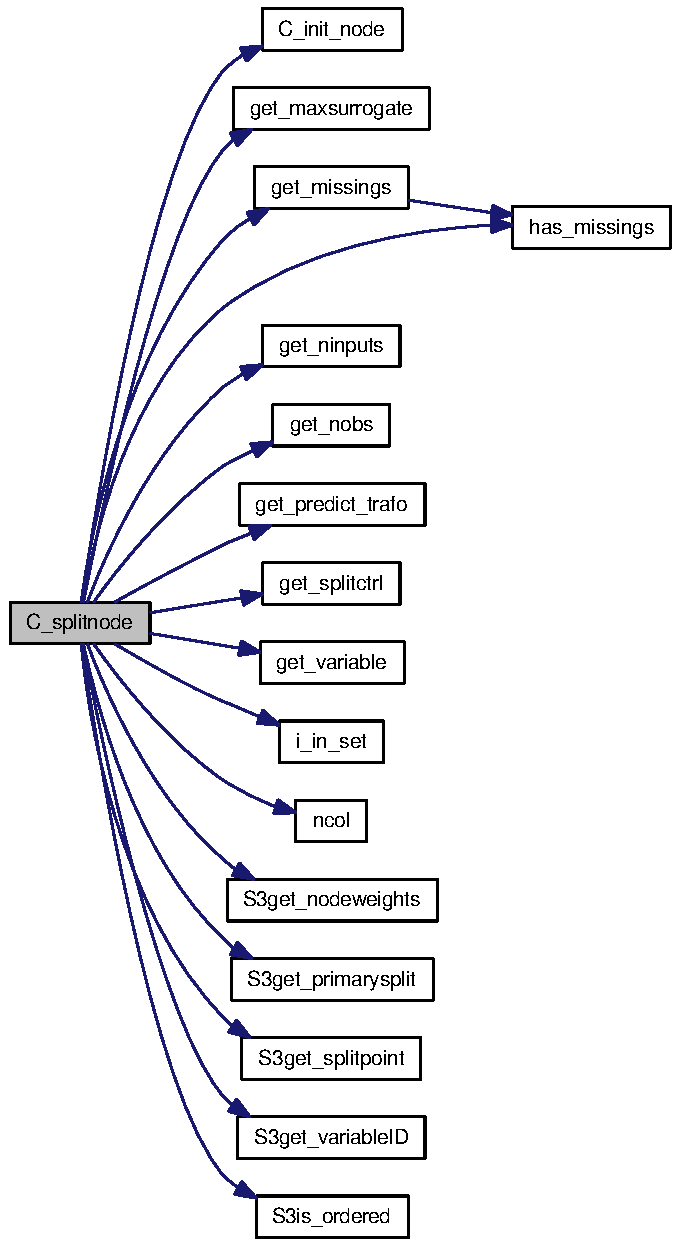
\includegraphics[width=181pt]{Predict_8c_daf8a0eb8790ebf14f0e265de164d50e_cgraph}
\end{center}
\end{figure}
\hypertarget{Predict_8c_dec31e3aa985e0af16ccaeac31237640}{
\index{Predict.c@{Predict.c}!R\_\-get\_\-node@{R\_\-get\_\-node}}
\index{R\_\-get\_\-node@{R\_\-get\_\-node}!Predict.c@{Predict.c}}
\subsubsection[R\_\-get\_\-node]{\setlength{\rightskip}{0pt plus 5cm}SEXP R\_\-get\_\-node (SEXP {\em subtree}, \/  SEXP {\em newinputs}, \/  SEXP {\em mincriterion}, \/  SEXP {\em numobs})}}
\label{Predict_8c_dec31e3aa985e0af16ccaeac31237640}


R-Interface to C\_\-get\_\-node \par
 \begin{Desc}
\item[Parameters:]
\begin{description}
\item[{\em subtree}]a tree \item[{\em newinputs}]an object of class `VariableFrame' \item[{\em mincriterion}]overwrites mincriterion used for tree growing \item[{\em numobs}]observation number \end{description}
\end{Desc}


Definition at line 230 of file Predict.c.

References C\_\-get\_\-node().

Here is the call graph for this function:\nopagebreak
\begin{figure}[H]
\begin{center}
\leavevmode
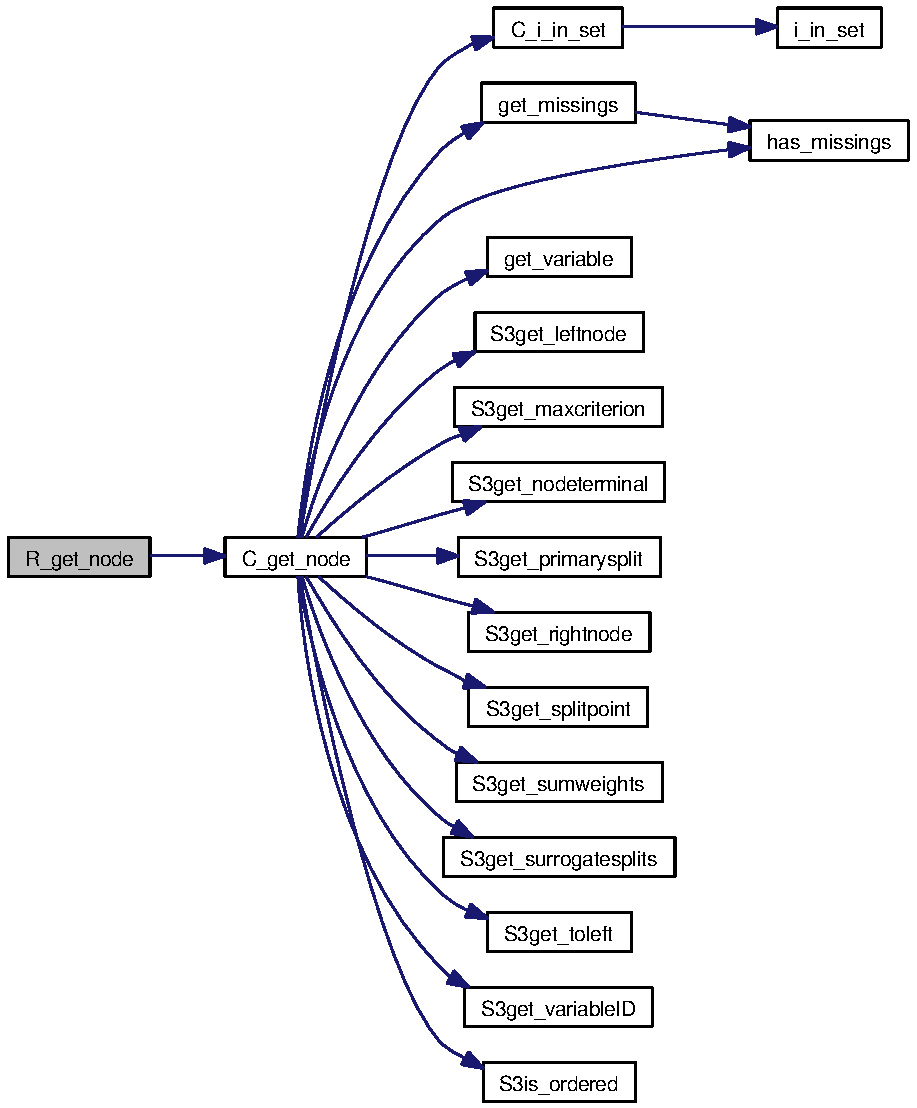
\includegraphics[width=238pt]{Predict_8c_dec31e3aa985e0af16ccaeac31237640_cgraph}
\end{center}
\end{figure}
\hypertarget{Predict_8c_4a30a8aa916f294059b6e2cbcb9e29d5}{
\index{Predict.c@{Predict.c}!R\_\-get\_\-nodebynum@{R\_\-get\_\-nodebynum}}
\index{R\_\-get\_\-nodebynum@{R\_\-get\_\-nodebynum}!Predict.c@{Predict.c}}
\subsubsection[R\_\-get\_\-nodebynum]{\setlength{\rightskip}{0pt plus 5cm}SEXP R\_\-get\_\-nodebynum (SEXP {\em subtree}, \/  SEXP {\em nodenum})}}
\label{Predict_8c_4a30a8aa916f294059b6e2cbcb9e29d5}


R-Interface to C\_\-get\_\-nodenum \par
 \begin{Desc}
\item[Parameters:]
\begin{description}
\item[{\em subtree}]a tree \item[{\em nodenum}]a nodeID \end{description}
\end{Desc}


Definition at line 264 of file Predict.c.

References C\_\-get\_\-nodebynum().

Here is the call graph for this function:\nopagebreak
\begin{figure}[H]
\begin{center}
\leavevmode
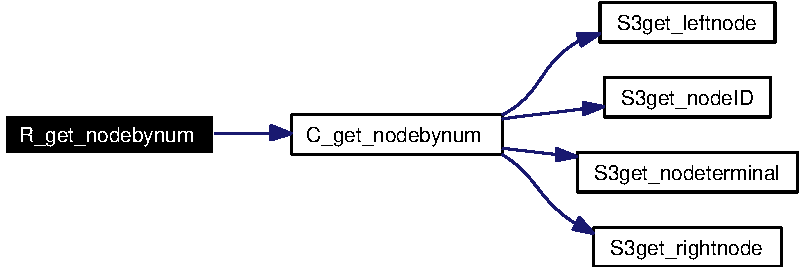
\includegraphics[width=207pt]{Predict_8c_4a30a8aa916f294059b6e2cbcb9e29d5_cgraph}
\end{center}
\end{figure}
\hypertarget{Predict_8c_c0668d268fe5a4bad29fbf4ead39c526}{
\index{Predict.c@{Predict.c}!R\_\-get\_\-nodeID@{R\_\-get\_\-nodeID}}
\index{R\_\-get\_\-nodeID@{R\_\-get\_\-nodeID}!Predict.c@{Predict.c}}
\subsubsection[R\_\-get\_\-nodeID]{\setlength{\rightskip}{0pt plus 5cm}SEXP R\_\-get\_\-nodeID (SEXP {\em tree}, \/  SEXP {\em newinputs}, \/  SEXP {\em mincriterion})}}
\label{Predict_8c_c0668d268fe5a4bad29fbf4ead39c526}


R-Interface to C\_\-get\_\-nodeID \par
 \begin{Desc}
\item[Parameters:]
\begin{description}
\item[{\em tree}]a tree \item[{\em newinputs}]an object of class `VariableFrame' \item[{\em mincriterion}]overwrites mincriterion used for tree growing \end{description}
\end{Desc}


Definition at line 321 of file Predict.c.

References C\_\-get\_\-nodeID(), and get\_\-nobs().

Here is the call graph for this function:\nopagebreak
\begin{figure}[H]
\begin{center}
\leavevmode
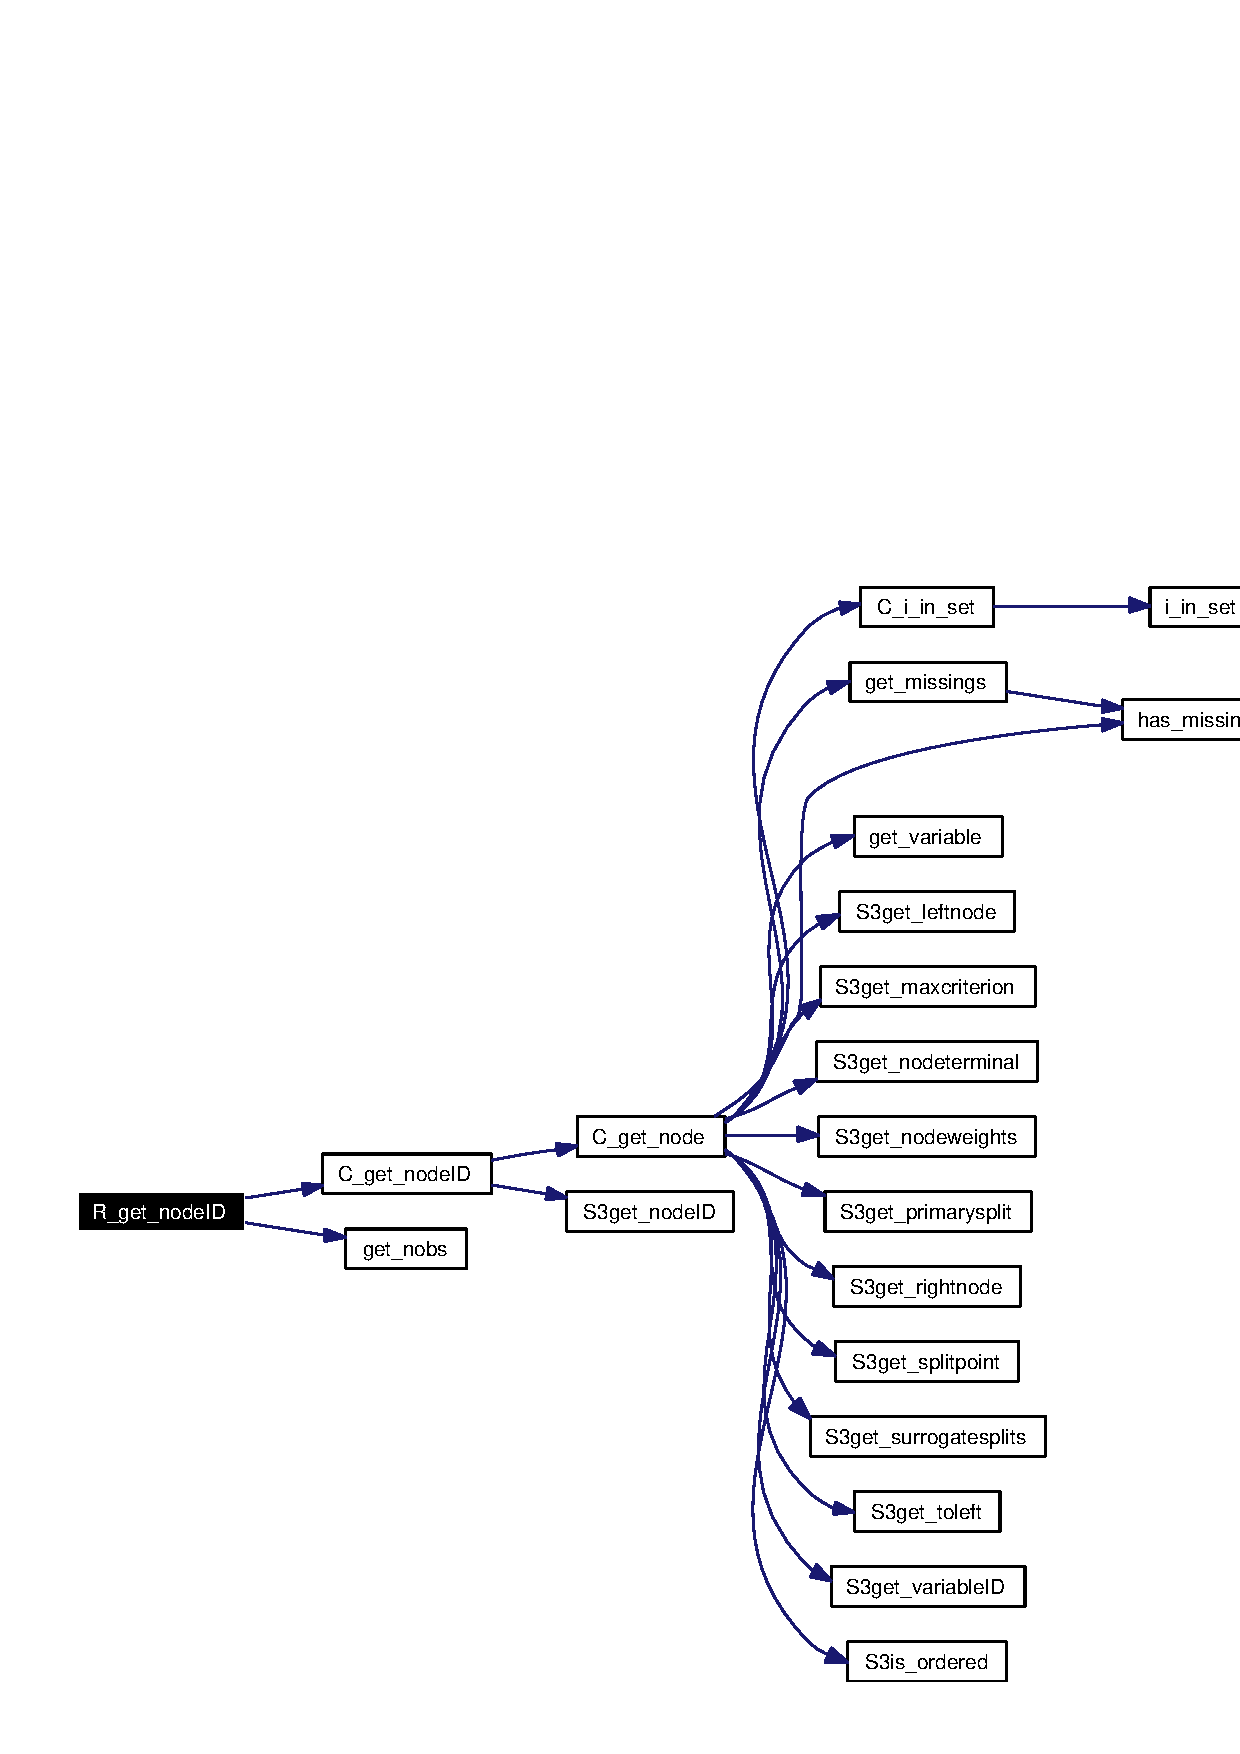
\includegraphics[width=305pt]{Predict_8c_c0668d268fe5a4bad29fbf4ead39c526_cgraph}
\end{center}
\end{figure}
\hypertarget{Predict_8c_a508a31f1fd7cd3668ad81eb0d00dd66}{
\index{Predict.c@{Predict.c}!R\_\-getpredictions@{R\_\-getpredictions}}
\index{R\_\-getpredictions@{R\_\-getpredictions}!Predict.c@{Predict.c}}
\subsubsection[R\_\-getpredictions]{\setlength{\rightskip}{0pt plus 5cm}SEXP R\_\-getpredictions (SEXP {\em tree}, \/  SEXP {\em where})}}
\label{Predict_8c_a508a31f1fd7cd3668ad81eb0d00dd66}


R-Interface to C\_\-getpredictions\par
 \begin{Desc}
\item[Parameters:]
\begin{description}
\item[{\em tree}]a tree \item[{\em where}]vector of nodeID's \end{description}
\end{Desc}


Definition at line 406 of file Predict.c.

References C\_\-getpredictions().

Here is the call graph for this function:\nopagebreak
\begin{figure}[H]
\begin{center}
\leavevmode
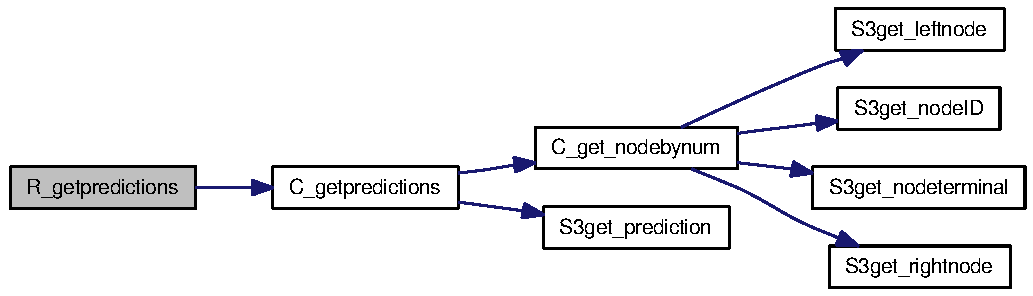
\includegraphics[width=266pt]{Predict_8c_a508a31f1fd7cd3668ad81eb0d00dd66_cgraph}
\end{center}
\end{figure}
\hypertarget{Predict_8c_9a5170a24bc00b727527b80cec5ca60a}{
\index{Predict.c@{Predict.c}!R\_\-predict@{R\_\-predict}}
\index{R\_\-predict@{R\_\-predict}!Predict.c@{Predict.c}}
\subsubsection[R\_\-predict]{\setlength{\rightskip}{0pt plus 5cm}SEXP R\_\-predict (SEXP {\em tree}, \/  SEXP {\em newinputs}, \/  SEXP {\em mincriterion})}}
\label{Predict_8c_9a5170a24bc00b727527b80cec5ca60a}


R-Interface to C\_\-predict \par
 \begin{Desc}
\item[Parameters:]
\begin{description}
\item[{\em tree}]a tree \item[{\em newinputs}]an object of class `VariableFrame' \item[{\em mincriterion}]overwrites mincriterion used for tree growing \end{description}
\end{Desc}


Definition at line 365 of file Predict.c.

References C\_\-predict(), and get\_\-nobs().

Here is the call graph for this function:\nopagebreak
\begin{figure}[H]
\begin{center}
\leavevmode
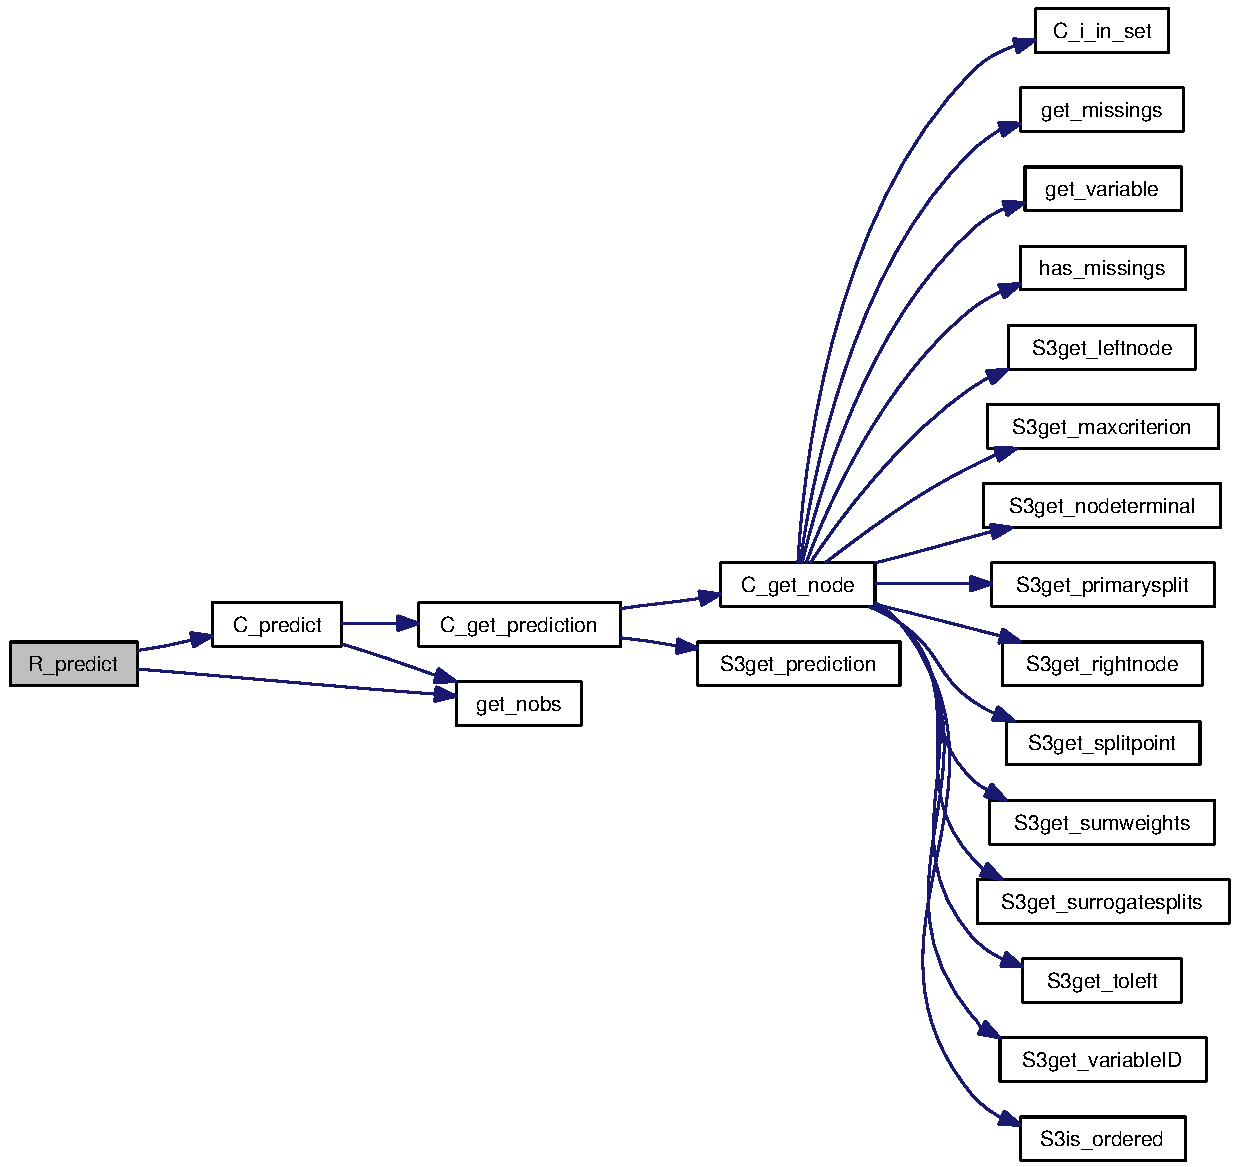
\includegraphics[width=354pt]{Predict_8c_9a5170a24bc00b727527b80cec5ca60a_cgraph}
\end{center}
\end{figure}
\hypertarget{Predict_8c_4f6966402677cec07284a3e1bc25660f}{
\index{Predict.c@{Predict.c}!R\_\-predictRF\_\-weights@{R\_\-predictRF\_\-weights}}
\index{R\_\-predictRF\_\-weights@{R\_\-predictRF\_\-weights}!Predict.c@{Predict.c}}
\subsubsection[R\_\-predictRF\_\-weights]{\setlength{\rightskip}{0pt plus 5cm}SEXP R\_\-predictRF\_\-weights (SEXP {\em forest}, \/  SEXP {\em where}, \/  SEXP {\em weights}, \/  SEXP {\em newinputs}, \/  SEXP {\em mincriterion}, \/  SEXP {\em oobpred})}}
\label{Predict_8c_4f6966402677cec07284a3e1bc25660f}


Predictions weights from RandomForest objects \begin{Desc}
\item[Parameters:]
\begin{description}
\item[{\em forest}]a list of trees \item[{\em where}]list (length b) of integer vectors (length n) containing terminal node numbers \item[{\em weights}]list (length b) of bootstrap case weights \item[{\em newinputs}]an object of class `VariableFrame' \item[{\em mincriterion}]overwrites mincriterion used for tree growing \item[{\em oobpred}]a logical indicating out-of-bag predictions \end{description}
\end{Desc}


Definition at line 428 of file Predict.c.

References C\_\-get\_\-nodebynum(), C\_\-get\_\-nodeID(), get\_\-nobs(), and S3get\_\-prediction().

Here is the call graph for this function:\nopagebreak
\begin{figure}[H]
\begin{center}
\leavevmode
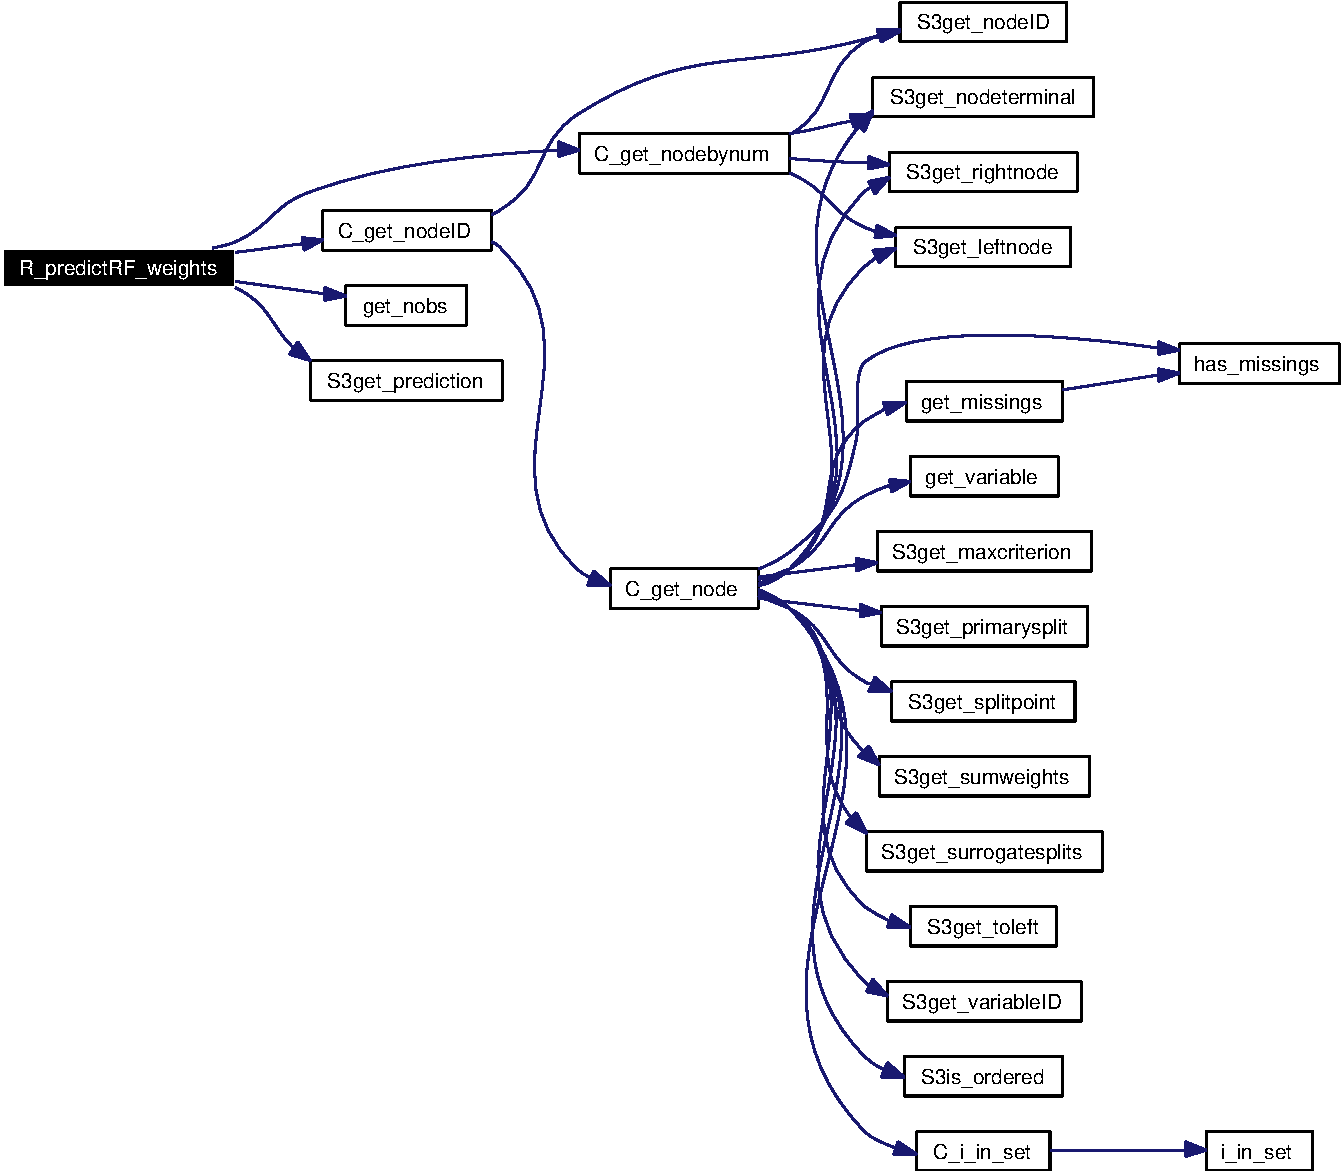
\includegraphics[width=336pt]{Predict_8c_4f6966402677cec07284a3e1bc25660f_cgraph}
\end{center}
\end{figure}
\hypertarget{Predict_8c_3be1a8f3155b0481350cecd4c094a416}{
\index{Predict.c@{Predict.c}!R\_\-proximity@{R\_\-proximity}}
\index{R\_\-proximity@{R\_\-proximity}!Predict.c@{Predict.c}}
\subsubsection[R\_\-proximity]{\setlength{\rightskip}{0pt plus 5cm}SEXP R\_\-proximity (SEXP {\em where})}}
\label{Predict_8c_3be1a8f3155b0481350cecd4c094a416}


Proximity matrix for random forests \begin{Desc}
\item[Parameters:]
\begin{description}
\item[{\em where}]list (length b) of integer vectors (length n) containing terminal node numbers \end{description}
\end{Desc}


Definition at line 484 of file Predict.c.